\chapter{Ajout d'une singularité dans le réseau}
La seconde partie de ce projet est une étude portant sur l'observation d'un mode localisé dans le réseau précédemment étudié. Pour cela, un résonateur est modifié de façon à créer une singularité dans le réseau. \\


Le banc de manipulation utilisé est le même que celui de la thèse~\cite{these_richoux} qui a servi de support au projet. Il ne permet de modifier que la longueur des cavités des résonateurs et non leur position. C'est donc en changeant ce paramètre que sera introduite et étudiée la singularité. La longueur de la cavité singulière est notée $L_{c_{s}}$.\\

En fonction du choix de la longueur de la cavité singulière, et donc de la fréquence de résonance du résonateur associé, différents phénomènes peuvent être observés. 

\section{Étude de l'influence de la fréquence de résonance du défaut}
Le réseau étudié a un comportement complexe d'un point de vue fréquentiel. Il est donc important de différentier les cas suivant la fréquence de résonance du défaut. Deux cas de figure sont représentés sur le schéma \ref{schema_singu1} : celui pour lequel la résonance du défaut est dans une bande interdite et celui où elle est dans une bande passante.

\begin{figure}[!h]
\centering
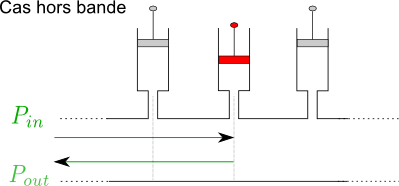
\includegraphics[scale=0.5]{images_chp2/schema_singu1.png} \hfill
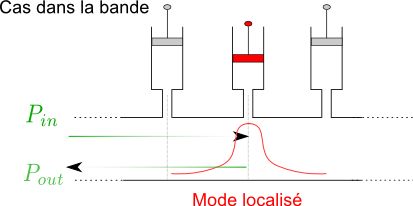
\includegraphics[scale=0.5]{images_chp2/schema_singu2.png}
\caption{\label{schema_singu1} Schémas de la configuration avec une singularité dans une bande interdite  et hors bande interdite.}
\end{figure}




\subsection{Cas du défaut hors bandes interdites}

Le cas le plus simple d'une singularité dans le réseau est celui ou cette singularité se trouve hors de la bande de Bragg ou des bandes liés aux autres résonateurs (la fréquence de résonance de la singularité est dans une bande passante). La singularité crée un changement d'impédance brutal dans le réseau à sa fréquence de résonance car alors l'impédance du résonateur est maximale. Dans ce cas, la pression dans le réseau après la singularité est nulle : l'onde est totalement réfléchie. Ce résultat est visible sur la figure~\ref{defaut_hb}. Cette figure est une simulation de l'amplitude de la pression dans le réseau, excité par un sinus à la fréquence de résonance du défaut.	Les lignes noires indiquent l'emplacement des résonateurs (de longueur de cavité 16 cm) et la ligne rouge indique l'emplacement du défaut de longueur de cavité 7.1 cm.

La pression est calculée en chaque point du réseau par rétro-propagation en partant d'une terminaison anéchoïque à la fin du réseau. Les amplitudes visible au niveau de la source n'ont donc pas nécessairement de réalité physique. On s'intéresse surtout à l'enveloppe du signal plus qu'aux ordres de grandeurs.


\begin{figure}[!h]
\centering
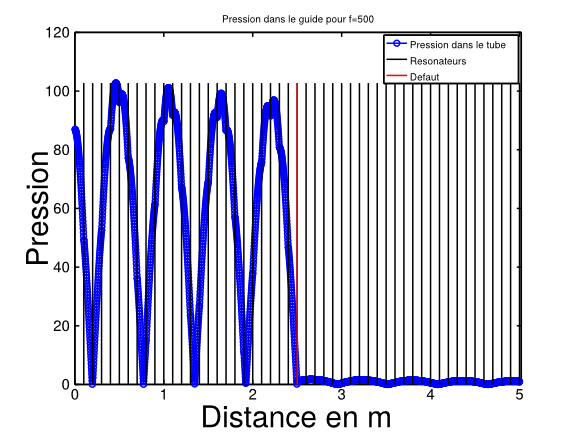
\includegraphics[scale=0.5]{images_chp2/horsbande_50RH_500Hz_71mm.png}
\caption{\label{defaut_hb} Visualisation de la pression dans le réseau avec un défaut dont la fréquence se trouve dans une bande passante. La fréquence d'excitation est celle du défaut (500 Hz). Celui-ci se trouve en 25\textsuperscript{ème} position dans un réseau de 50 résonateurs espacés de 10 cm.}
\end{figure}

\bigskip
On constate bien une chute de la pression au niveau de la singularité. Le défaut a théoriquement une impédance infinie à la résonance, il y a donc une réflexion totale. Ici, les pertes sont prisent en compte : une fraction de l'onde incidente se propage donc dans le réseau après le défaut.



\subsection{Cas du défaut dans une bande interdite}

Si la fréquence de résonance du défaut se trouve dans une bande interdite, on a alors une localisation de l'onde au niveau du défaut. En effet, la propagation n'est pas possible de part et d'autre du défaut dans le réseau (ondes évanescentes). La fraction de l'onde incidente qui s'est propagée jusqu'au défaut excite ce dernier mais reste piégée du fait que ce défaut se trouve au milieu du réseau. On obtient alors un mode localisé : la pression est élevée à un endroit du guide et y reste confinée.
\bigskip


Du fait que cette pression soit localisée, elle n'a pas d'influence sur le coefficient de transmission sauf dans le cas d'un petit réseau où l'on peut supposer que l'étalement du mode localisé est suffisamment grand au regard de la taille du réseau pour atteindre les bords de celui-ci. Ce genre de phénomène est donc difficile à observer; cependant une simulation peut aider à en comprendre les concepts clés.
\bigskip

Comme précédemment, on trace sur la figure \ref{defaut_dansb} la pression dans le tube pour un défaut dont la résonance se trouve dans une bande interdite. Le réseau est excité à la fréquence du mode localisé. Cette fréquence résulte d'un couplage entre la singularité et le réseau. Elle peut être retrouvée expérimentalement car c'est la fréquence à laquelle la pression est maximale au niveau de la singularité. Elle peut aussi se retrouver sur le coefficient de réflexion : comme le montre la courbe de droite de la figure~\ref{defaut_dansb}, le coefficient de réflexion est très faible pour une fréquence donnée au milieu de la bande interdite. Cette fréquence correspond à celle du mode recherché.


\begin{figure}[!h]
\centering
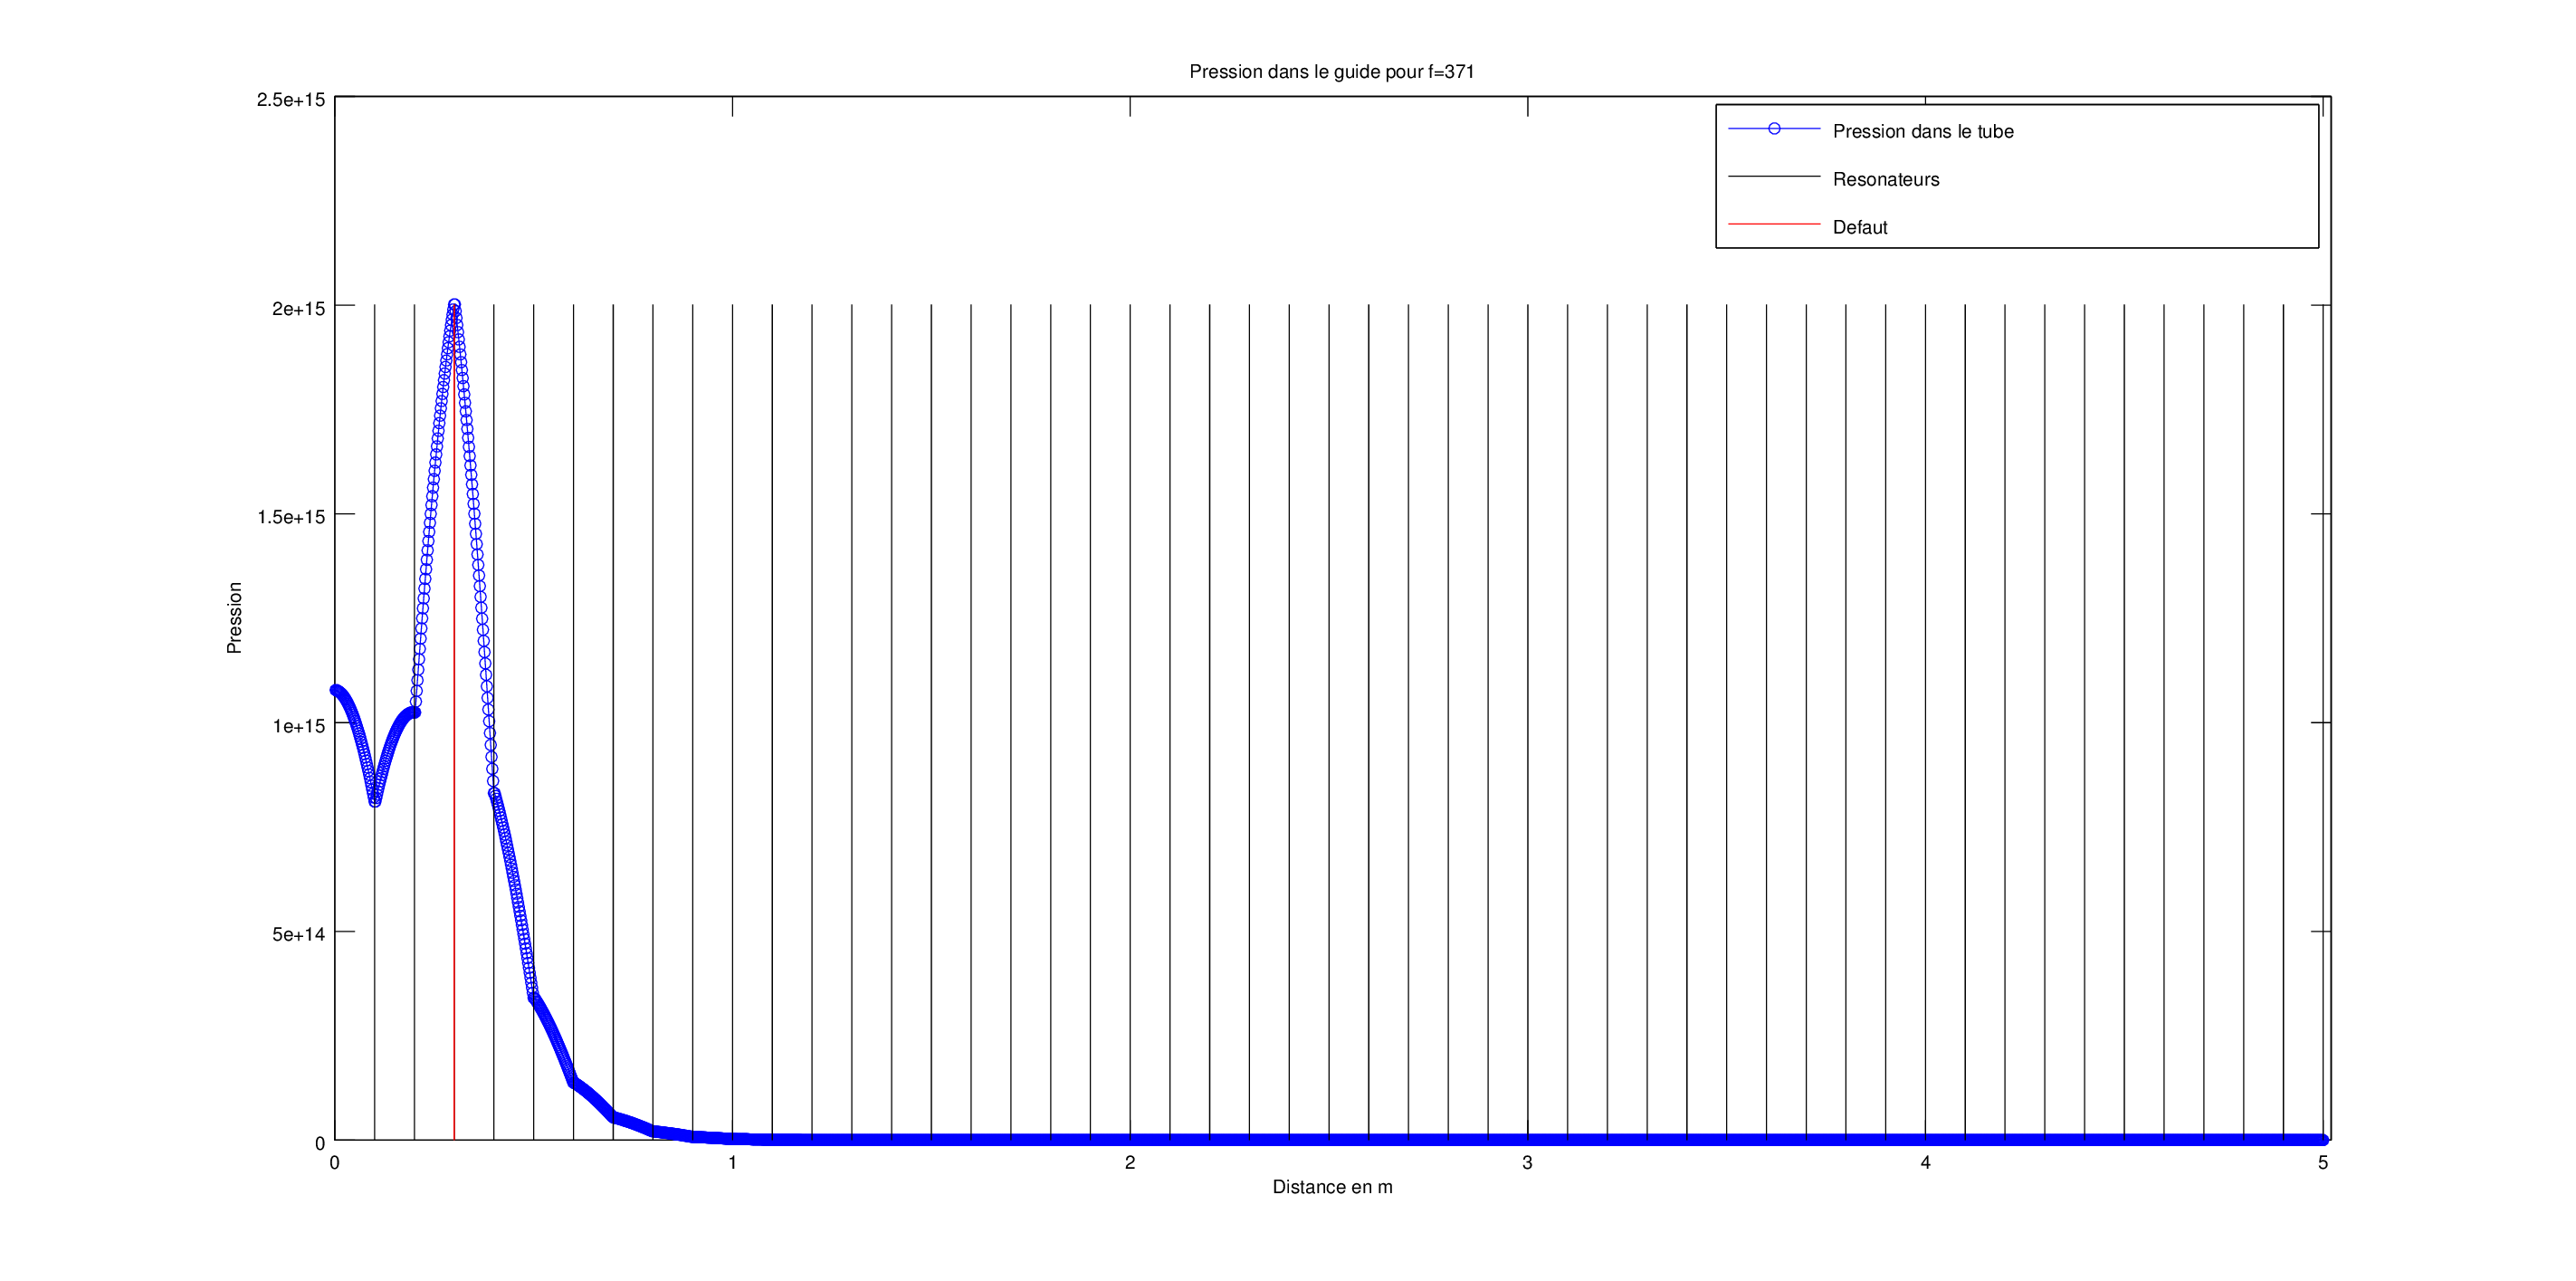
\includegraphics[width=0.6 \textwidth]{images_chp2/visu_pression_favo2.png}
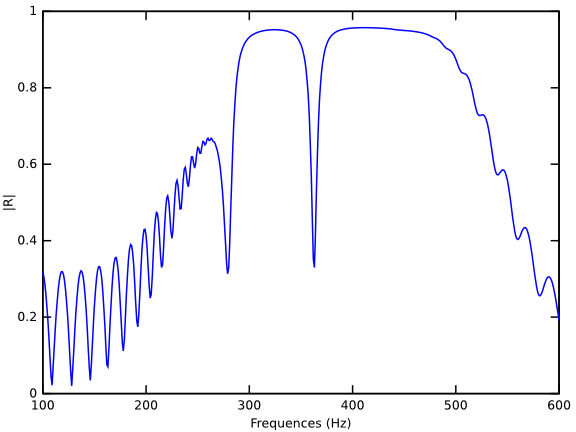
\includegraphics[width=0.35 \textwidth]{images_chp2/reflexion_50HR16_pos3_8cm.png}
\caption{\label{defaut_dansb} À gauche : Visualisation de la pression dans le réseau avec un défaut dont la fréquence se trouve dans une bande interdite ($L_{c_{s}}=8cm$. La fréquence d'excitation est à 371 Hz. Le défaut se trouve en 3\textsuperscript{ème} position dans un réseau de 50 résonateurs espacés de 10 cm.\\ À droite : Coefficient de réflexion pour le même réseau.}
\end{figure}



\section{Étude de l'influence de la position du défaut}
La position du défaut est elle aussi très importante afin de pouvoir générer un mode localisé: le défaut doit être suffisamment proche de la source afin d'être excité par les ondes évanescentes mais pas trop proche des bords car alors il n'est plus complètement localisé.

La figure~\ref{pos_singu} représente le coefficient de transmission pour un réseau constitué de 5 résonateurs en fonction de la position du défaut ($L_{c_{s}}=6.5 cm$). Il apparaît clairement que quand le défaut est en position 2 ou 3, une hausse de la transmission est visible autour de 390 Hz. Cette fréquence est celle du mode localisé. 

\begin{figure}
	\centering
	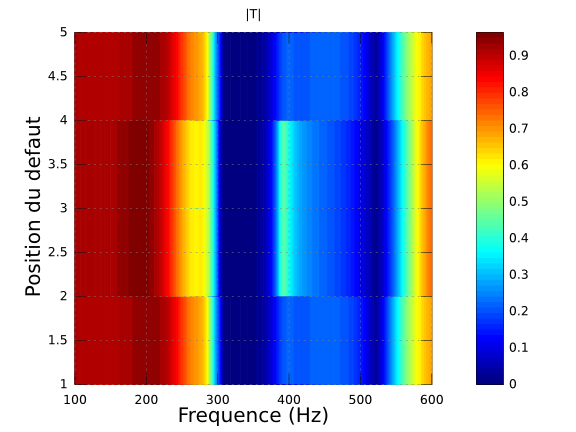
\includegraphics[scale=0.5]{images_chp2/pos_singu.png}
	\caption{Coefficient de transmission en fonction de la position du défaut et de la fréquence d'excitation.\label{pos_singu}}
\end{figure}

Dans la partie suivante, l'objectif est de visualiser expérimentalement ce mode localisé. Cette simulation numérique montre donc qu'il faut choisir judicieusement la position du résonateur défectueux ainsi que la fréquence d'excitation du réseau.